\documentclass[12pt,a4paper]{article}
\usepackage[margin=1in]{geometry}
\usepackage{array}
\usepackage{fancyhdr}
\usepackage{tikz}
\usepackage{amsmath}
\usepackage{enumitem}
\raggedbottom
\usepackage{float}

\pagestyle{fancy}
\fancyhf{}
\rhead{Physics (PH)}
\renewcommand{\headrulewidth}{0pt}

\usepackage{amsmath, amssymb}
\usepackage{geometry}
\usepackage{array}
\usepackage{booktabs}
\usepackage{tabularx}
\usepackage{tikz}
\usepackage{pgfplots}
\pgfplotsset{compat=1.18}
\usetikzlibrary{arrows.meta, decorations.markings}

\geometry{top=2cm, bottom=2cm, left=2.5cm, right=2.5cm}

\setlength{\arrayrulewidth}{0.5pt}
\renewcommand{\arraystretch}{1.6}

\newcolumntype{L}{>{\raggedright\arraybackslash}p{1.2cm}}
\newcolumntype{C}{>{\raggedright\arraybackslash}p{13cm}}

\begin{document}

% --------- PAGE 1: Q.1 ---------
\begin{center}
    \textbf{\underline{General Aptitude (GA)}}
\end{center}

\textbf{Q.1 -- Q.5 Carry ONE mark Each}

\vspace{0.5em}

\begin{tabular}{|p{1cm}|p{12cm}|}
\hline
Q.1 & ``He often \underline{\hspace{1.5cm}} the numbers. False claims are not going to help. Honesty \underline{\hspace{1.5cm}} trust'', said the manager. \\
    & \\
    & Choose the option with the correct order of words to fill the blanks. \\
\hline
(A) & exaggerates; engenders \\
\hline
(B) & excels; encourages \\
\hline
(C) & aggravates; alleviates \\
\hline
(D) & diminishes; eliminates \\
\hline
& \rule{0pt}{8cm} \\
\hline
\end{tabular}

\newpage

% --------- PAGE 2: Q.2 ---------
\begin{tabular}{|p{1cm}|p{12cm}|}
\hline
Q.2 & In the sequence of tiles shown below, the missing tile indicated by the question mark should be \\
    & \\
    & \hspace{1em}
    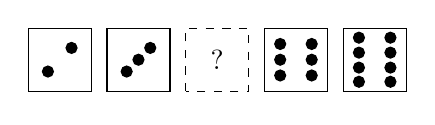
\begin{tikzpicture}[baseline=-0.5ex]
      % Tile 1: 2 dots
      \draw (0,0) rectangle (0.8,0.8);
      \filldraw (0.55,0.55) circle (0.07);
      \filldraw (0.25,0.25) circle (0.07);
      % Tile 2: 3 dots
      \draw (1.0,0) rectangle (1.8,0.8);
      \filldraw (1.55,0.55) circle (0.07);
      \filldraw (1.40,0.40) circle (0.07);
      \filldraw (1.25,0.25) circle (0.07);
      % Tile 3: ? dashed
      \draw[dashed] (2.0,0) rectangle (2.8,0.8);
      \node at (2.4,0.4) {?};
      % Tile 4: 6 dots
      \draw (3.0,0) rectangle (3.8,0.8);
      \filldraw (3.2,0.6) circle (0.07); \filldraw (3.6,0.6) circle (0.07);
      \filldraw (3.2,0.4) circle (0.07); \filldraw (3.6,0.4) circle (0.07);
      \filldraw (3.2,0.2) circle (0.07); \filldraw (3.6,0.2) circle (0.07);
      % Tile 5: 8 dots
      \draw (4.0,0) rectangle (4.8,0.8);
      \filldraw (4.2,0.68) circle (0.07); \filldraw (4.6,0.68) circle (0.07);
      \filldraw (4.2,0.49) circle (0.07); \filldraw (4.6,0.49) circle (0.07);
      \filldraw (4.2,0.30) circle (0.07); \filldraw (4.6,0.30) circle (0.07);
      \filldraw (4.2,0.12) circle (0.07); \filldraw (4.6,0.12) circle (0.07);
    \end{tikzpicture} \\
\hline
& \rule{0pt}{0.8cm} \\
\hline
(A) & \rule{0pt}{1.2cm} 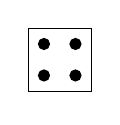
\begin{tikzpicture}[baseline=-0.5ex]
      \draw (0,0) rectangle (0.8,0.8);
      \filldraw (0.2,0.6) circle (0.07); \filldraw (0.6,0.6) circle (0.07);
      \filldraw (0.2,0.2) circle (0.07); \filldraw (0.6,0.2) circle (0.07);
    \end{tikzpicture} \\
\hline
(B) & \rule{0pt}{1.2cm} 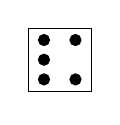
\begin{tikzpicture}[baseline=-0.5ex]
      \draw (0,0) rectangle (0.8,0.8);
      \filldraw (0.2,0.65) circle (0.07); \filldraw (0.6,0.65) circle (0.07);
      \filldraw (0.2,0.40) circle (0.07);
      \filldraw (0.2,0.15) circle (0.07); \filldraw (0.6,0.15) circle (0.07);
    \end{tikzpicture} \\
\hline
(C) & \rule{0pt}{1.2cm} 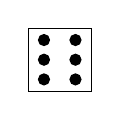
\begin{tikzpicture}[baseline=-0.5ex]
      \draw (0,0) rectangle (0.8,0.8);
      \filldraw (0.2,0.65) circle (0.07); \filldraw (0.6,0.65) circle (0.07);
      \filldraw (0.2,0.40) circle (0.07); \filldraw (0.6,0.40) circle (0.07);
      \filldraw (0.2,0.15) circle (0.07); \filldraw (0.6,0.15) circle (0.07);
    \end{tikzpicture} \\
\hline
(D) & \rule{0pt}{1.2cm} 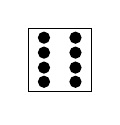
\begin{tikzpicture}[baseline=-0.5ex]
      \draw (0,0) rectangle (0.8,0.8);
      \filldraw (0.2,0.68) circle (0.07); \filldraw (0.6,0.68) circle (0.07);
      \filldraw (0.2,0.49) circle (0.07); \filldraw (0.6,0.49) circle (0.07);
      \filldraw (0.2,0.30) circle (0.07); \filldraw (0.6,0.30) circle (0.07);
      \filldraw (0.2,0.12) circle (0.07); \filldraw (0.6,0.12) circle (0.07);
    \end{tikzpicture} \\
\hline
& \rule{0pt}{0.8cm} \\
\hline
\end{tabular}

\newpage

% --------- PAGE 3: Q.3 & Q.4 ---------
\begin{tabular}{|p{1cm}|p{12cm}|}
\hline
Q.3 & A school has 100 students distributed among 1\textsuperscript{st} to 10\textsuperscript{th} standards. \\
    & \\
    & Based on this, which one of the following statements is always correct? \\
\hline
& \rule{0pt}{0.8cm} \\
\hline
(A) & There are at least 10 students who belong to the same standard. \\
\hline
(B) & There is at least one student in each standard. \\
\hline
(C) & There are at most 10 students in 10\textsuperscript{th} standard. \\
\hline
(D) & The total number of students from 1\textsuperscript{st} to 5\textsuperscript{th} standards is at least 50. \\
\hline
& \rule{0pt}{0.8cm} \\
\hline
\end{tabular}

\vspace{1em}

\begin{tabular}{|p{1cm}|p{12cm}|}
\hline
Q.4 & How many 3-digit numbers can be formed using three distinct single digit prime numbers? \\
\hline
& \rule{0pt}{0.8cm} \\
\hline
(A) & 64 \\
\hline
(B) & 24 \\
\hline
(C) & 12 \\
\hline
(D) & 4 \\
\hline
& \rule{0pt}{0.8cm} \\
\hline
\end{tabular}

\newpage

% --------- PAGE 4: Q.5 ---------
\begin{tabular}{|p{1cm}|p{12cm}|}
\hline
Q.5 & In a group of students, 10 students like Mathematics, 12 students like English, 4 students like both Mathematics and English, and 6 students like neither Mathematics nor English. The number of students in the group is \underline{\hspace{1cm}} \\
\hline
& \rule{0pt}{0.8cm} \\
\hline
(A) & 18 \\
\hline
(B) & 20 \\
\hline
(C) & 24 \\
\hline
(D) & 32 \\
\hline
& \rule{0pt}{0.8cm} \\
\hline
\end{tabular}

\newpage

% --------- PAGE 5: Q.6 ---------
\textbf{Q.6 -- Q.10 Carry TWO marks Each}

\vspace{0.5em}

\begin{tabular}{|p{1cm}|p{12cm}|}
\hline
Q.6 & Charity : P :: Retaliation : Q \\
    & \\
    & Choose the appropriate pair of words P and Q that fit the analogy. \\
\hline
& \rule{0pt}{0.8cm} \\
\hline
(A) & P = Parsimonious; Q = Vengeful \\
\hline
(B) & P = Altruistic; Q = Amicable \\
\hline
(C) & P = Resentful; Q = Spiteful \\
\hline
(D) & P = Magnanimous; Q = Vindictive \\
\hline
& \rule{0pt}{8cm} \\
\hline
\end{tabular}

\newpage

% --------- PAGE 6: Q.7 ---------
\newpage
% --------- PAGE 6: Q.7 ---------
\begin{tabular}{|p{1cm}|p{12cm}|}
\hline
Q.7 & A paper shown in Panel I is folded along the dashed lines (- - -) to construct a cube. The shaded regions shown in Panel I appear on the outer surface of the cube. Referring to cubes shown in Panel II, which one of the options is correct? \\
    & \\
    & \begin{minipage}{12cm}
        \centering
        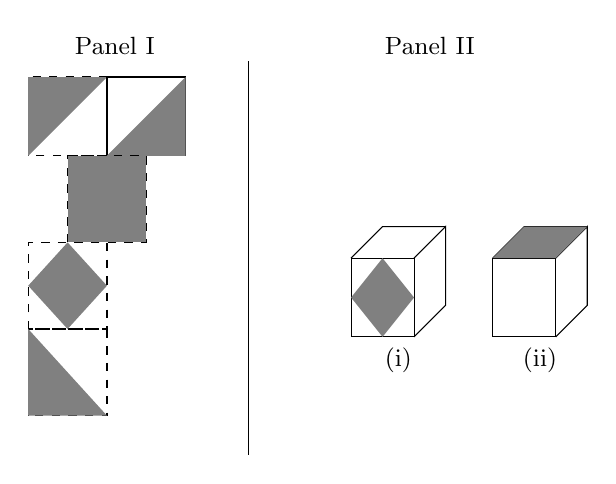
\begin{tikzpicture}
          \node at (1.5, 5.2) {\small Panel I};
          \node at (5.5, 5.2) {\small Panel II};
          \draw (3.2, 0.0) -- (3.2, 5.0);
          % Panel I
          \draw[dashed] (0.4,3.8) rectangle (1.4,4.8);
          \fill[gray] (0.4,4.8) -- (1.4,4.8) -- (0.4,3.8) -- cycle;
          \draw (1.4,3.8) rectangle (2.4,4.8);
          \fill[gray] (1.4,3.8) -- (2.4,3.8) -- (2.4,4.8) -- cycle;
          \draw[dashed] (0.9,2.7) rectangle (1.9,3.8);
          \fill[gray] (0.9,2.7) rectangle (1.9,3.8);
          \draw[dashed] (0.4,1.6) rectangle (1.4,2.7);
          \fill[gray] (0.9,1.6) -- (1.4,2.15) -- (0.9,2.7) -- (0.4,2.15) -- cycle;
          \draw[dashed] (0.4,0.5) rectangle (1.4,1.6);
          \fill[gray] (0.4,0.5) -- (1.4,0.5) -- (0.4,1.6) -- cycle;
          % Panel II cube (i)
          \draw (4.5,1.5) -- (5.3,1.5) -- (5.3,2.5) -- (4.5,2.5) -- cycle;
          \draw (5.3,1.5) -- (5.7,1.9) -- (5.7,2.9) -- (5.3,2.5);
          \draw (4.5,2.5) -- (4.9,2.9) -- (5.7,2.9);
          \fill[gray] (4.9,1.5) -- (5.3,2.0) -- (4.9,2.5) -- (4.5,2.0) -- cycle;
          \node at (5.1,1.2) {\small (i)};
          % Panel II cube (ii)
          \draw (6.3,1.5) -- (7.1,1.5) -- (7.1,2.5) -- (6.3,2.5) -- cycle;
          \draw (7.1,1.5) -- (7.5,1.9) -- (7.5,2.9) -- (7.1,2.5);
          \draw (6.3,2.5) -- (6.7,2.9) -- (7.5,2.9);
          \fill[gray] (6.3,2.5) -- (6.7,2.9) -- (7.5,2.9) -- (7.1,2.5) -- cycle;
          \node at (6.9,1.2) {\small (ii)};
        \end{tikzpicture}
      \end{minipage} \\
\hline
& \rule{0pt}{0.8cm} \\
\hline
(A) & Only (i) can correspond to the unfolded cube in Panel I. \\
\hline
(B) & Only (ii) can correspond to the unfolded cube in Panel I. \\
\hline
(C) & Both (i) and (ii) can correspond to the unfolded cube in Panel I. \\
\hline
(D) & Neither (i) nor (ii) can correspond to the unfolded cube in Panel I. \\
\hline
& \rule{0pt}{0.8cm} \\
\hline
\end{tabular}

\newpage

% --------- PAGE 7: Q.8 ---------
\begin{tabular}{|p{1cm}|p{12cm}|}
\hline
Q.8 & Consider the cube shown below with its 8 corners labelled a, b, c, d, e, f, g and h. The figure is representative. All corners are to be colored such that any two corners that are connected by an edge must be of different colors. The minimum number of colors required to achieve this is \underline{\hspace{1.5cm}} \\
    & \\
    & \begin{center}
      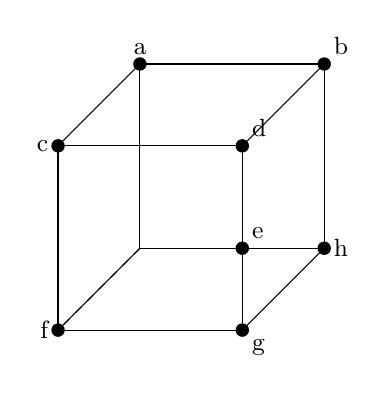
\begin{tikzpicture}[scale=1.3]
        % Back face
        \draw (1.0,2.0) -- (2.8,2.0) -- (2.8,3.8) -- (1.0,3.8) -- cycle;
        % Front face
        \draw (0.2,1.2) -- (2.0,1.2) -- (2.0,3.0) -- (0.2,3.0) -- cycle;
        % Connecting edges
        \draw (0.2,1.2) -- (1.0,2.0);
        \draw (2.0,1.2) -- (2.8,2.0);
        \draw (2.0,3.0) -- (2.8,3.8);
        \draw (0.2,3.0) -- (1.0,3.8);
        % Corners and labels
        % a: top-left back
        \filldraw (1.0,3.8) circle (0.06); \node[above] at (1.0,3.8) {\small a};
        % b: top-right back
        \filldraw (2.8,3.8) circle (0.06); \node[above right] at (2.8,3.8) {\small b};
        % c: top-left front
        \filldraw (0.2,3.0) circle (0.06); \node[left] at (0.2,3.0) {\small c};
        % d: top-right front (inner top)
        \filldraw (2.0,3.0) circle (0.06); \node[above right] at (2.0,3.0) {\small d};
        % e: bottom-left front (inner)
        \filldraw (2.0,2.0) circle (0.06); \node[above right] at (2.0,2.0) {\small e};
        % h: right front bottom
        \filldraw (2.8,2.0) circle (0.06); \node[right] at (2.8,2.0) {\small h};
        % f: bottom-left front
        \filldraw (0.2,1.2) circle (0.06); \node[left] at (0.2,1.2) {\small f};
        % g: bottom-right front
        \filldraw (2.0,1.2) circle (0.06); \node[below right] at (2.0,1.2) {\small g};
        % Hidden edges (dashed)
        \draw[dashed] (1.0,2.0) -- (2.8,2.0);
        \draw[dashed] (1.0,2.0) -- (1.0,3.8);
        \draw[dashed] (1.0,2.0) -- (0.2,1.2);
      \end{tikzpicture}
      \end{center} \\
\hline
& \rule{0pt}{0.8cm} \\
\hline
(A) & 8 \\
\hline
(B) & 4 \\
\hline
(C) & 3 \\
\hline
(D) & 2 \\
\hline
& \rule{0pt}{4cm} \\
\hline
\end{tabular}


\newpage

% --------- PAGE 8: Q.9 ---------
\begin{tabular}{|p{1cm}|p{12cm}|}
\hline
Q.9 & Four hills H1, H2, H3, and H4 are present in an area. The following observations
are made about them:
\begin{enumerate}[i.]
    \item Neither H2 nor H3 is the easternmost hill.
    \item Neither H2 nor H3 is the westernmost hill.
    \item Neither the easternmost hill nor the westernmost hill is the southernmost hill.
    \item Two hills are located to the west of H2.
    \item The southernmost hill has at least two hills to its east.
\end{enumerate}
The southernmost hill is \underline{\hspace{1.5cm}}. \\
\hline
& \rule{0pt}{0.8cm} \\
\hline
(A) & H1 \\
\hline
(B) & H2 \\
\hline
(C) & H3 \\
\hline
(D) & H4 \\
\hline
& \rule{0pt}{0.8cm} \\
\hline
\end{tabular}

\vspace{1em}

% --------- Q.10 ---------
\begin{tabular}{|p{1cm}|p{12cm}|}
\hline
Q.10 & As shown in the figure, circle $C_1$ with center $O_1$ and radius $r_1$ touches the square $VWXY$ at points $P$ and $Q$ while circle $C_2$ with center $O_2$ and radius $r_2$ touches the square $VWXY$ at points $R$ and $S$. The two circles touch each other at $T$. \\
     & Given $r_1 = 1$ cm and $\overline{VY} = \overline{VW} = 4$ cm, $r_2 =$ \underline{\hspace{1cm}} cm. \\
       & \centering
       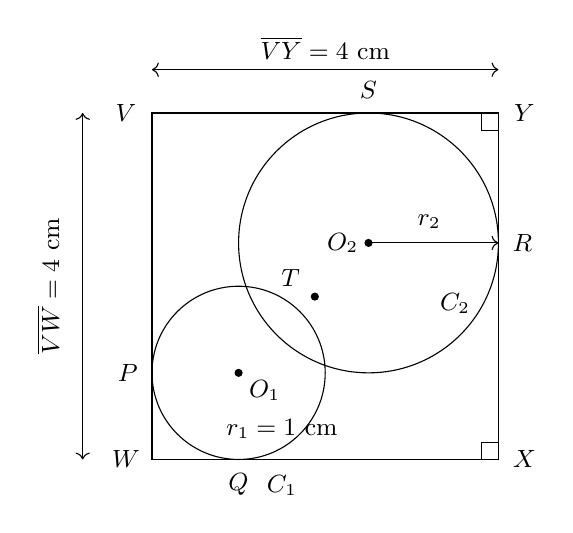
\begin{tikzpicture}[scale=1.1]
         \draw (0,0) rectangle (4,4);
         \node at (-0.3, 4.0) {\small $V$};
         \node at ( 4.3, 4.0) {\small $Y$};
         \node at (-0.3, 0.0) {\small $W$};
         \node at ( 4.3, 0.0) {\small $X$};
         \draw (3.8,0) rectangle (4.0,0.2);
         \draw (3.8,3.8) rectangle (4.0,4.0);
         \draw[<->] (0,4.5) -- (4,4.5);
         \node at (2,4.75) {\small $\overline{VY} = 4$ cm};
         \draw[<->] (-0.8,0) -- (-0.8,4);
         \node[rotate=90] at (-1.2,2) {\small $\overline{VW} = 4$ cm};
         % Circle C1
         \draw (1,1) circle (1);
         \filldraw (1,1) circle (0.04);
         \node at (1.3,0.8) {\small $O_1$};
         \node at (1.5,0.35) {\small $r_1 = 1$ cm};
         \node at (1.5,-0.3) {\small $C_1$};
         \node[below] at (1,-0.05) {\small $Q$};
         \node[left]  at (-0.05,1) {\small $P$};
         % Circle C2
         \draw (2.5,2.5) circle (1.5);
         \filldraw (2.5,2.5) circle (0.04);
         \node at (2.2,2.5) {\small $O_2$};
         \node at (3.5,1.8) {\small $C_2$};
         \node at (3.2,2.75) {\small $r_2$};
         \draw[->] (2.5,2.5) -- (4,2.5);
         \node[right] at (4.05,2.5) {\small $R$};
         \node[above] at (2.5,4.05) {\small $S$};
         % Touch point T
         \filldraw (1.88,1.88) circle (0.04);
         \node at (1.6,2.1) {\small $T$};
       \end{tikzpicture} \\
       
& \rule{0pt}{0.8cm} \\
\hline
(A) & $4 - 3\sqrt{2}$ \\
\hline
(B) & $1 + 2\sqrt{2}$ \\
\hline
(C) & $7 - 4\sqrt{2}$ \\
\hline
(D) & $5 + 3\sqrt{2}$ \\
\hline
& \rule{0pt}{0.8cm} \\
\hline
\end{tabular}

\newpage

% --------- PAGE 10: Q.11 & Q.12 ---------
\textbf{Q.11 -- Q.35 Carry ONE mark Each}

\vspace{0.5em}

\begin{tabular}{|p{1cm}|p{12cm}|}
\hline
Q.11 & In free space, an electromagnetic wave is travelling whose wavevector is
$\vec{k} = 10(\hat{z} + \sqrt{3}\hat{y})$ m$^{-1}$. The electric field component of this electromagnetic wave is
given by $\vec{E}(\vec{r},t) = \hat{z}\, 600\cos(\vec{k}\cdot\vec{r} - \omega t)$ V.m$^{-1}$. The speed of light in free space is
$c = 3.0 \times 10^8$ m.s$^{-1}$. The corresponding magnetic field $\vec{B}(\vec{r},t)$ is \\
\hline
& \rule{0pt}{0.8cm} \\
\hline
(A) & $\vec{B}(\vec{r},t) = 2 \times 10^{-6}(\sqrt{3}\hat{x} - \hat{y})\cos(\vec{k}\cdot\vec{r} - \omega t)$ V.m$^{-2}$.s \\
\hline
(B) & $\vec{B}(\vec{r},t) = 10^{-6}(\sqrt{3}\hat{x} - \hat{y})\cos(\vec{k}\cdot\vec{r} - \omega t)$ V.m$^{-2}$.s \\
\hline
(C) & $\vec{B}(\vec{r},t) = 2 \times 10^{-6}(-\sqrt{3}\hat{x} + \hat{y})\cos(\vec{k}\cdot\vec{r} - \omega t)$ V.m$^{-2}$.s \\
\hline
(D) & $\vec{B}(\vec{r},t) = 10^{-5}(\sqrt{3}\hat{x} - \hat{y})\cos(\vec{k}\cdot\vec{r} - \omega t)$ V.m$^{-2}$.s \\
\hline
& \rule{0pt}{0.8cm} \\
\hline
\end{tabular}

\vspace{1em}

\begin{tabular}{|p{1cm}|p{12cm}|}
\hline
Q.12 & An infinitely large non-conducting thin sheet in the $xy$ plane ($z{=}0$) carries a uniform
surface charge density $\sigma = 17.70 \times 10^{-12}$ C.m$^{-2}$. The electric field in the region $z < 0$
is $\vec{E}_2 = \hat{x} + 2\hat{y} + 3\hat{z}$. Then, the electric field $\vec{E}_1$ in the region $z > 0$ will be \\
& \\
& $(\varepsilon_0 = 8.85 \times 10^{-12}$ C$^2$.N$^{-1}$.m$^{-2})$ \\
\hline
& \rule{0pt}{0.8cm} \\
\hline
(A) & $\vec{E}_1 = \hat{x} + 2\hat{y} + 5\hat{z}$ \\
\hline
(B) & $\vec{E}_1 = \hat{x} + 2\hat{y} + 4\hat{z}$ \\
\hline
(C) & $\vec{E}_1 = \hat{x} + 2\hat{y} + 3\hat{z}$ \\
\hline
(D) & $\vec{E}_1 = \hat{x} + 4\hat{y} + \hat{z}$ \\
\hline
& \rule{0pt}{0.8cm} \\
\hline
\end{tabular}

\newpage

% --------- PAGE 11: Q.13 ---------
\begin{tabular}{|p{1cm}|p{12cm}|}
\hline
Q.13 & Consider an operator $\hat{A}$ which is not Hermitian. Find the possible values of $c$ and $d$ such
that the operator $(c\,\hat{A} - d\,\hat{A}^\dagger)$ is Hermitian. \\
\hline
& \rule{0pt}{0.8cm} \\
\hline
(A) & $c = i$ and $d = i$ \\
\hline
(B) & $c = 1$ and $d = 1$ \\
\hline
(C) & $c = -1$ and $d = i$ \\
\hline
(D) & $c = i$ and $d = -i$ \\
\hline
& \rule{0pt}{0.8cm} \\
\hline
\end{tabular}

\newpage

% --------- PAGE 12: Q.14 & Q.15 ---------
\begin{tabular}{|p{1cm}|p{12cm}|}
\hline
Q.14 & For a scalar field $\psi(\vec{r})$ and a vector field $\vec{A}(\vec{r})$,
$\vec{\nabla} \times (\vec{A}\,\psi)$ is equivalent to the expression \\
\hline
& \rule{0pt}{0.8cm} \\
\hline
(A) & $\psi(\vec{\nabla} \times \vec{A}) - \vec{A} \times (\vec{\nabla}\psi)$ \\
\hline
(B) & $\psi(\vec{\nabla} \times \vec{A}) + \vec{A} \times (\vec{\nabla}\psi)$ \\
\hline
(C) & Null vector \\
\hline
(D) & $\vec{A} \times (\vec{\nabla}\psi) - \psi(\vec{\nabla} \times \vec{A})$ \\
\hline
& \rule{0pt}{0.8cm} \\
\hline
\end{tabular}

\vspace{1em}

\begin{tabular}{|p{1cm}|p{12cm}|}
\hline
Q.15 & Which of the following options is correct for transformation of electric field $\vec{E}$ and
magnetic field $\vec{B}$ under time reversal, i.e., $t \to -t$\,? \\
\hline
& \rule{0pt}{0.8cm} \\
\hline
(A) & $\vec{E} \to \vec{E}$ and $\vec{B} \to \vec{B}$ \\
\hline
(B) & $\vec{E} \to -\vec{E}$ and $\vec{B} \to \vec{B}$ \\
\hline
(C) & $\vec{E} \to \vec{E}$ and $\vec{B} \to -\vec{B}$ \\
\hline
(D) & $\vec{E} \to -\vec{E}$ and $\vec{B} \to -\vec{B}$ \\
\hline
& \rule{0pt}{0.8cm} \\
\hline
\end{tabular}

\newpage

% --------- PAGE 13: Q.16 ---------
\begin{tabular}{|p{1cm}|p{12cm}|}
\hline
Q.16 & On a horizontal plane, a projectile of mass $m$ is launched from the ground with speed $v_0$
at an angle $\theta_0$ with the horizontal. In addition to the gravitational force ($mg$), it also
experiences a drag force $\vec{F}_{drag} = -\gamma\vec{v}$, where $\vec{v}$ is its velocity and $\gamma$ is a constant.
It hits the ground at a distance $R$ from the point of launch with its velocity making an angle
$\theta$ with the horizontal, as shown schematically in the figure. Then which of the following
options is correct? \\
& \\
& \centering
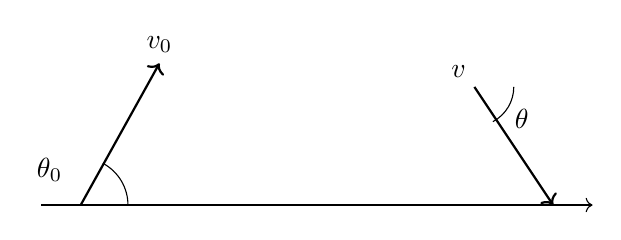
\begin{tikzpicture}[scale=1.0]
  \draw[->] (0,0) -- (7,0);
  \draw[->, thick] (0.5,0) -- (1.5,1.8) node[above] {$v_0$};
  \draw (0.5,0) ++(0:0.6) arc (0:62:0.6);
  \node at (0.105,0.45) {$\theta_0$};
  \draw[->, thick] (5.5,1.5) -- (6.5,0);
  \node at (5.3,1.7) {$v$};
  \draw (5.5,1.5) ++(-62:0.5) arc (-62:0:0.5);
  \node at (6.1,1.1) {$\theta$};
  \draw (0.5,0) -- (6.5,0);
\end{tikzpicture} \\
& \rule{0pt}{0.8cm} \\
\hline
(A) & \rule{0pt}{1.2cm} $R = \dfrac{v_0^2 \sin 2\theta}{g}$ \qquad $\theta < \theta_0$ \\[0.5em]
\hline
(B) & \rule{0pt}{1.2cm} $R < \dfrac{v_0^2 \sin 2\theta_0}{g}$ \qquad $\theta < \theta_0$ \\[0.5em]
\hline
(C) & \rule{0pt}{1.2cm} $R < \dfrac{v_0^2 \sin 2\theta_0}{g}$ \qquad $\theta > \theta_0$ \\[0.5em]
\hline
(D) & \rule{0pt}{1.2cm} $R = \dfrac{v_0^2 \sin 2\theta}{g}$ \qquad $\theta > \theta_0$ \\[0.5em]
\hline
& \rule{0pt}{5cm} \\
\hline
\end{tabular}

\newpage

% --------- PAGE 14: Q.17 ---------
\begin{tabular}{|p{1cm}|p{12cm}|}
\hline
Q.17 & Consider the Otto cycle for an ideal gas engine consisting of two quasistatic adiabatic and
two quasistatic isochoric processes. The correct temperature-entropy (T-S) phase diagram
for the cycle is \\
\hline
& \rule{0pt}{0.8cm} \\
\hline
(A) & 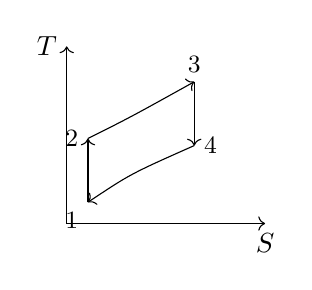
\begin{tikzpicture}[scale=0.9]
  \draw[->] (0,0) -- (0,2.5) node[left] {$T$};
  \draw[->] (0,0) -- (2.8,0) node[below] {$S$};
  \coordinate (P1) at (0.3,0.3);
  \coordinate (P2) at (0.3,1.2);
  \coordinate (P3) at (1.8,2.0);
  \coordinate (P4) at (1.8,1.1);
  \draw[->] (P1) -- (P2) node[left] {\small 2};
  \draw[->] (P2) .. controls (0.9,1.5) .. (P3) node[above] {\small 3};
  \draw[->] (P3) -- (P4) node[right] {\small 4};
  \draw[->] (P4) .. controls (0.9,0.7) .. (P1);
  \node[below left] at (P1) {\small 1};
\end{tikzpicture} \\
\hline
(B) & 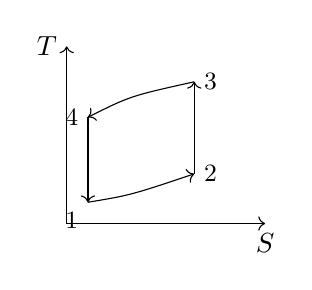
\begin{tikzpicture}[scale=0.9]
  \draw[->] (0,0) -- (0,2.5) node[left] {$T$};
  \draw[->] (0,0) -- (2.8,0) node[below] {$S$};
  \coordinate (P1) at (0.3,0.3);
  \coordinate (P2) at (1.8,0.7);
  \coordinate (P3) at (1.8,2.0);
  \coordinate (P4) at (0.3,1.5);
  \draw[->] (P1) .. controls (0.9,0.4) .. (P2) node[right] {\small 2};
  \draw[->] (P2) -- (P3) node[right] {\small 3};
  \draw[->] (P3) .. controls (0.9,1.8) .. (P4) node[left] {\small 4};
  \draw[->] (P4) -- (P1);
  \node[below left] at (P1) {\small 1};
\end{tikzpicture} \\
\hline
(C) & \begin{tikzpicture}[scale=0.9]
  \draw[->] (0,0) -- (0,2.5) node[left] {$T$};
  \draw[->] (0,0) -- (2.8,0) node[below] {$S$};
  \coordinate (P1) at (0.3,0.3);
  \coordinate (P2) at (0.3,1.5);
  \coordinate (P3) at (1.8,1.5);
  \coordinate (P4) at (1.8,0.3);
  \draw[->] (P1) -- (P2) node[left] {\small 2};
  \draw[->] (P2) -- (P3) node[above] {\small 3};
  \draw[->] (P3) -- (P4) node[right] {\small 4};
  \draw[->] (P4) -- (P1);
  \node[below left] at (P1) {\small 1};
\end{tikzpicture} \\
\hline
(D) & \begin{tikzpicture}[scale=0.9]
  \draw[->] (0,0) -- (0,2.5) node[left] {$T$};
  \draw[->] (0,0) -- (2.8,0) node[below] {$S$};
  \coordinate (P1) at (0.3,0.3);
  \coordinate (P2) at (1.8,0.3);
  \coordinate (P3) at (1.8,1.5);
  \coordinate (P4) at (0.3,1.5);
  \draw[->] (P1) -- (P2) node[below] {\small 2};
  \draw[->] (P2) -- (P3) node[right] {\small 3};
  \draw[->] (P3) -- (P4) node[above] {\small 4};
  \draw[->] (P4) -- (P1);
  \node[below left] at (P1) {\small 1};
\end{tikzpicture} \\
\hline
& \rule{0pt}{0.8cm} \\
\hline
\end{tabular}

\newpage

% --------- PAGE 15: Q.18 & Q.19 ---------
\begin{tabular}{|p{1cm}|p{12cm}|}
\hline
Q.18 & The formula for energy $E$ of a photon gas at temperature $T$ in a two-dimensional box at
equilibrium with $g_{2d}(\nu)$ denoting the density of states of photons is given below where
symbols $\nu$, $h$ and $k_B$ have their standard meaning. The specific heat ($C_V$) of this photon
gas obeys
$E = \int_0^{\infty} d\nu\, g_{2d}(\nu)\, \dfrac{h\nu}{\exp\!\left(\dfrac{h\nu}{k_B T}\right) - 1}$ \\
\hline
& \rule{0pt}{0.8cm} \\
\hline
(A) & $C_V \propto T$ \\
\hline
(B) & $C_V \propto T^2$ \\
\hline
(C) & $C_V \propto T^3$ \\
\hline
(D) & $C_V \propto T^4$ \\
\hline
& \rule{0pt}{0.8cm} \\
\hline
\end{tabular}

\vspace{1em}

\begin{tabular}{|p{1cm}|p{12cm}|}
\hline
Q.19 & For the electric field of an electromagnetic wave given below, which of the following
statements is correct?
$\vec{E} = \hat{x}\, E_0 \cos(\omega t) + \hat{y}\, 2E_0 \cos\!\left(\omega t + \dfrac{\pi}{2}\right)$ \\
\hline
& \rule{0pt}{0.8cm} \\
\hline
(A) & The electric field is linearly polarised with slope 2. \\
\hline
(B) & The electric field is circularly polarised with radius $E_0$. \\
\hline
(C) & The electric field is elliptically polarised with a ratio of major to minor axis being 2. \\
\hline
(D) & The electric field is unpolarised with the two components being phase shifted by $\pi/2$. \\
\hline
& \rule{0pt}{0.8cm} \\
\hline
\end{tabular}

\newpage

% --------- PAGE 16: Q.20 & Q.21 ---------
\begin{tabular}{|p{1cm}|p{12cm}|}
\hline
Q.20 & A gas of non-interacting $^4$He atoms (of mass $m$) is in a three-dimensional trap whose
energy levels can be approximated by those of a harmonic oscillator potential
$V(x,y,z) = \frac{1}{2}m\omega^2(x^2 + y^2 + z^2)$. The chemical potential of the gas at $T{=}0$ K is \\
\hline
& \rule{0pt}{0.8cm} \\
\hline
(A) & \rule{0pt}{2em}$0$ \\[0.5em]
\hline
(B) & \rule{0pt}{2.5em}$\dfrac{1}{2}\hbar\omega$ \\[0.5em]
\hline
(C) & \rule{0pt}{2.5em}$\dfrac{3}{2}\hbar\omega$ \\[0.5em]
\hline
(D) & \rule{0pt}{2em}$3\hbar\omega$ \\[0.5em]
\hline
& \rule{0pt}{0.8cm} \\
\hline
\end{tabular}

\newpage
\vspace{1em}

\begin{tabular}{|p{1cm}|p{12cm}|}
\hline
Q.21 & Given $|v_1\rangle = \dfrac{1}{\sqrt{2}}\left(\begin{smallmatrix}1\\i\end{smallmatrix}\right)$
and $|v_2\rangle = \dfrac{1}{\sqrt{2}}\left(\begin{smallmatrix}1\\-i\end{smallmatrix}\right)$,
the tensor product $|v_1\rangle \otimes |v_2\rangle$ is \\
\hline
& \rule{0pt}{0.8cm} \\
\hline
(A) & \rule{0pt}{5em}$\dfrac{1}{2}\left(\begin{array}{c}1\\-i\\i\\1\end{array}\right)$ \\[4em]
\hline
(B) & \rule{0pt}{5em}$\dfrac{1}{2}\left(\begin{array}{c}1\\i\\-i\\1\end{array}\right)$ \\[4em]
\hline
(C) & \rule{0pt}{4em}$\dfrac{1}{2}\left(\begin{array}{cc}1 & i\\i & -1\end{array}\right)$ \\[3em]
\hline
(D) & \rule{0pt}{4em}$\dfrac{1}{2}\left(\begin{array}{cc}1 & i\\-i & 1\end{array}\right)$ \\[3em]
\hline
& \rule{0pt}{0.8cm} \\
\hline
\end{tabular}

\newpage
%% ─────────────────────────────────────────────
%%  Q.22
%% ─────────────────────────────────────────────
\begin{table}[h!]
\begin{tabular}{|L|C|}
\hline
Q.22 &
Sketch of a two-dimensional vector field $\vec{V}$ is shown below. Here, length and
arrow head of the arrows denote magnitude and direction of the vector field,
respectively. Which of the following statements is correct for $\vec{\nabla} \times \vec{V}$\,?

\vspace{0.4cm}

% ── Vector field diagram ──────────────────────
\begin{center}
\begin{tikzpicture}[scale=0.72,
  arr/.style={-{Stealth[length=4pt]}, thin}
]

% Draw axes
\draw[->] (-4.2,0) -- (4.5,0) node[right] {$x$};
\draw[->] (0,-2.5) -- (0,2.8) node[above] {$y$};

% Helper macro: \hv{x}{y}{len}  draws a horizontal arrow of half-length len centred at (x,y)
% Arrows point in +x direction; length proportional to |y| (longer away from x-axis)
% Above x-axis: longer arrows; below: same pattern mirrored

% Row y = 2
\foreach \x in {-3.5,-2.5,-1.5,-0.5,0.5,1.5,2.5,3.5}{
  \pgfmathsetmacro\len{0.55}
  \draw[arr] (\x-\len,2) -- (\x+\len,2);
}

% Row y = 1
\foreach \x in {-3.5,-2.5,-1.5,-0.5,0.5,1.5,2.5,3.5}{
  \pgfmathsetmacro\len{0.35}
  \draw[arr] (\x-\len,1) -- (\x+\len,1);
}

% Row y = 0  (zero length — just dots or tiny arrows)
\foreach \x in {-3.5,-2.5,-1.5,-0.5,0.5,1.5,2.5,3.5}{
  \fill (\x,0) circle (1.2pt);
}

% Row y = -1
\foreach \x in {-3.5,-2.5,-1.5,-0.5,0.5,1.5,2.5,3.5}{
  \pgfmathsetmacro\len{0.35}
  \draw[arr] (\x-\len,-1) -- (\x+\len,-1);
}

% Row y = -2
\foreach \x in {-3.5,-2.5,-1.5,-0.5,0.5,1.5,2.5,3.5}{
  \pgfmathsetmacro\len{0.55}
  \draw[arr] (\x-\len,-2) -- (\x+\len,-2);
}

\end{tikzpicture}
\end{center}
\\
\hline
 & \\
\hline
(A) & It is zero everywhere in the two-dimensional space. \\
\hline
(B) & Its magnitude is non-zero and its direction is out of the two-dimensional plane. \\
\hline
(C) & Its magnitude is non-zero and its direction is into the two-dimensional plane. \\
\hline
(D) & It points in opposite directions above and below the $x$-axis. \\
\hline
 & \\
\hline
\end{tabular}
\end{table}

\vspace{0.5cm}

%% ─────────────────────────────────────────────
%%  Q.23
%% ─────────────────────────────────────────────
\begin{table}[h!]
\begin{tabular}{|L|C|}
\hline
Q.23 & Which one of the following is an allowed process? \\
\hline
 & \\
\hline
(A) & $\pi^- + p \;\to\; \pi^0 + n$ \\
\hline
(B) & $\pi^0 \;\to\; \gamma + \gamma + \gamma$ \\
\hline
(C) & $p + \bar{p} \;\to\; \Lambda^0 + \Lambda^0$ \\
\hline
(D) & $p + \bar{p} \;\to\; \gamma$ \\
\hline
 & \\
\hline
\end{tabular}
\end{table}

\newpage

%% ─────────────────────────────────────────────
%%  Q.24
%% ─────────────────────────────────────────────
\begin{table}[h!]
\begin{tabular}{|L|C|}
\hline
Q.24 &
Given $Q$ is the electromagnetic charge and $S$ is the strangeness quantum number,
identify the particle(s) for which $(Q - S) = 0$ is satisfied. \\
\hline
 & \\
\hline
(A) & $\Sigma^{-}$ \\
\hline
(B) & $K^{+}$ \\
\hline
(C) & $\Omega^{-}$ \\
\hline
(D) & $\Delta^{++}$ \\
\hline
 & \\
\hline
\end{tabular}
\end{table}

\vspace{0.8cm}

\newpage

%% ─────────────────────────────────────────────
%%  Q.25
%% ─────────────────────────────────────────────
\begin{table}[h!]
\begin{tabular}{|L|C|}
\hline
Q.25 &
Schematic variation of the specific heat $C_p$ of an ideal gas of diatomic molecules
with temperature $T$ is shown in the figure below. For rotational energy $E_R$ and
vibrational energy $E_v$ of the molecule, which of the following options is/are
correct? Here $k_B$ is the Boltzmann constant.

\vspace{0.4cm}

% ── Cp vs T diagram ───────────────────────────
\begin{center}
\begin{tikzpicture}[scale=1.0]

\begin{axis}[
  width=8cm, height=6cm,
  axis lines=left,
  xlabel={$T$},
  ylabel={$C_p$},
  xmin=0, xmax=10,
  ymin=0, ymax=5,
  xtick={3,6},
  xticklabels={$T_1$,$T_2$},
  ytick=\empty,
  xlabel style={at={(axis description cs:1,0)}, anchor=west},
  ylabel style={at={(axis description cs:0,1)}, anchor=south},
  clip=false,
  tick style={draw=none},
  axis line style={-{Stealth[length=5pt]}},
]

% Flat region 1 (low T, translational only)
\addplot[black, thick, domain=0:2.2] {1.5};

% First sigmoid rise (rotational modes activated, around T1)
\addplot[black, thick, domain=2.2:3.8,samples=60]
  {1.5 + 1.0/(1+exp(-3*(x-3)))};

% Flat region 2 (translational + rotational)
\addplot[black, thick, domain=3.8:5.2] {2.5};

% Second sigmoid rise (vibrational modes activated, around T2)
\addplot[black, thick, domain=5.2:6.8,samples=60]
  {2.5 + 1.0/(1+exp(-3*(x-6)))};

% Flat region 3 (fully active)
\addplot[black, thick, domain=6.8:9.5] {3.5};

% Dashed vertical lines at T1 and T2
\draw[dashed] (axis cs:3,0) -- (axis cs:3,2.5);
\draw[dashed] (axis cs:6,0) -- (axis cs:6,3.5);

\end{axis}
\end{tikzpicture}
\end{center}
\\
\hline
 & \\
\hline
(A) & $E_R \cong k_B T_1$ \\
\hline
(B) & $E_R \cong k_B T_2$ \\
\hline
(C) & $E_v \cong k_B T_1$ \\
\hline
(D) & $E_v \cong k_B T_2$ \\
\hline
 & \\
\hline
\end{tabular}
\end{table}

\newpage
%% ─────────────────────────────────────────────
%%  Q.26
%% ─────────────────────────────────────────────
\begin{table}[h!]
\begin{tabular}{|L|C|}
\hline
Q.26 &
If the perturbation $V = \lambda x^3$ is added to the Hamiltonian of a one-dimensional
harmonic oscillator, the matrix element $\langle m|V|0\rangle$ is/are non-zero for which
of the following states?

\medskip
Here, the eigenstates of the harmonic oscillator are denoted by $|n\rangle$. \\
\hline
 & \\
\hline
(A) & $|m = 3\rangle$ \\
\hline
(B) & $|m = 1\rangle$ \\
\hline
(C) & $|m = 2\rangle$ \\
\hline
(D) & $|m = 5\rangle$ \\
\hline
 & \\
\hline
\end{tabular}
\end{table}

\vspace{0.4cm}

%% ─────────────────────────────────────────────
%%  Q.27
%% ─────────────────────────────────────────────
\begin{table}[h!]
\begin{tabular}{|L|C|}
\hline
Q.27 & For which of the following functions does the Laplacian vanish? \\
\hline
 & \\
\hline
(A) & $x e^{y} - y e^{x}$ \\[8pt]
\hline
(B) & $x\cos(y) - y\cos(x)$ \\[8pt]
\hline
(C) & $e^{x+iy}$ \\[8pt]
\hline
(D) & \rule{0pt}{1.2cm}$yx^{2} - \dfrac{y^{3}}{3} - xy$ \\[8pt]
\hline
 & \\
\hline
\end{tabular}
\end{table}

\newpage
\vspace{0.4cm}

%% ─────────────────────────────────────────────
%%  Q.28
%% ─────────────────────────────────────────────
\begin{table}[h!]
\begin{tabular}{|L|C|}
\hline
Q.28 &
A projectile of mass $m$ is launched from the ground with the initial speed $v_0$ at an
angle $30^\circ$ from the horizontal. Take the ground to be horizontal. Ignoring the
drag, the magnitude of Hamilton's action $\int L\,dt$ for the particle from the beginning
till it hits the ground is $f \times \!\left(\dfrac{mv_0^2}{g}\right)$. The value of $f$
(rounded off to two decimal places) is \underline{\hspace{1.5cm}} \\
\hline
\end{tabular}
\end{table}

\vspace{0.4cm}

%% ─────────────────────────────────────────────
%%  Q.29
%% ─────────────────────────────────────────────
\begin{table}[h!]
\begin{tabular}{|L|C|}
\hline
Q.29 &
Consider an electron in the energy eigenstate $\psi_{211}(\vec{r})$ of the hydrogen atom.
Given that the radial probability distribution of the electron in such a state takes its
maximum value at $r = n_0\,a$, where $a$ is the Bohr radius, and $n_0$ is an integer.
The value of $n_0$ (in integer) is \underline{\hspace{1.5cm}}

\medskip
The radial part of the wavefunction $\psi_{211}(\vec{r})$ is given by
$R_{21}(r) = \dfrac{1}{\sqrt{24a^3}}\,r\,e^{-r/2a}$. \\
\hline
\end{tabular}
\end{table}

\vspace{0.4cm}

%% ─────────────────────────────────────────────
%%  Q.30
%% ─────────────────────────────────────────────
\begin{table}[h!]
\begin{tabular}{|L|C|}
\hline
Q.30 &
A dielectric sphere carries a uniform polarization $P = 26\;\mu\text{C}\cdot\text{cm}^{-2}$.
The magnitude of the electric field at the center of the sphere is
$E \times 10^{9}\;\text{N}\cdot\text{C}^{-1}$. The value of $E$ (rounded off to one
decimal place) is \underline{\hspace{1.5cm}}

\medskip
$(\varepsilon_0 = 8.85 \times 10^{-12}\;\text{C}^2\cdot\text{N}^{-1}\cdot\text{m}^{-2})$ \\
\hline
\end{tabular}
\end{table}

\vspace{0.4cm}

%% ─────────────────────────────────────────────
%%  Q.31
%% ─────────────────────────────────────────────
\begin{table}[h!]
\begin{tabular}{|L|C|}
\hline
Q.31 &
Consider a metal--superconductor junction connected to a dc voltage $V$. At $T < T_c$,
where $T_c$ is the superconductor's transition temperature, the current $I$ versus $V$
behavior of this junction is shown schematically in the figure below. If the
superconducting energy gap is $D$ meV, the value of $D$ (rounded off to one decimal
place) is \underline{\hspace{1.5cm}}

\vspace{0.4cm}

\begin{center}
\begin{tikzpicture}[scale=1.05]
  \draw[->] (0,0) -- (5.5,0) node[right] {$V$};
  \draw[->] (0,0) -- (0,3.5) node[above] {$I$};
  \node[below left] at (0,0) {$(0,0)$};
  % threshold tick
  \draw (2.0, 0.06) -- (2.0,-0.06);
  \node[below] at (2.0,0) {\small $V_{Th} = 1.0\;\text{mV}$};
  % zero-current region
  \draw[thick] (0,0) -- (2.0,0);
  % linear rise
  \draw[thick] (2.0,0) -- (4.8,3.0);
  % label
  \node at (2.8,2.0) {\small $T < T_c$};
\end{tikzpicture}
\end{center}
\\
\hline
\end{tabular}
\end{table}

\vspace{0.4cm}

%% ─────────────────────────────────────────────
%%  Q.32
%% ─────────────────────────────────────────────
\begin{table}[h!]
\begin{tabular}{|L|C|}
\hline
Q.32 &
For the energy dispersion of an electron in a one-dimensional solid
\[
  E(k) = E_0 - 2\gamma\cos(ka),
\]
the ratio of the effective mass of the electron in the solid to the free electron mass
$(m_e)$ at $k = 0$ is $R_0$. Taking $\gamma = 0.5\;\text{eV}$ and $a = 0.5\;\text{nm}$,
the value of $R_0$ (rounded off to two decimal places) is \underline{\hspace{1.5cm}}

\medskip
$(\hbar = 1.054\times10^{-34}\;\text{J}\cdot\text{s},\;
  m_e = 9.1\times10^{-31}\;\text{kg},\;
  \text{electron charge} = 1.6\times10^{-19}\;\text{C})$ \\
\hline
\end{tabular}
\end{table}

\vspace{0.4cm}

%% ─────────────────────────────────────────────
%%  Q.33
%% ─────────────────────────────────────────────
\begin{table}[h!]
\begin{tabular}{|L|C|}
\hline
Q.33 &
The specific heat $C_p(T)$ of one mole of a material as a function of temperature $T$ is
given as $C_p(T) = AT + BT^{-3}$, where $A = 0.695\;\text{mJ}\cdot\text{mol}^{-1}
\cdot\text{K}^{-2}$ and $B = 0.045\;\text{mJ}\cdot\text{mol}^{-1}\cdot\text{K}^{4}$.
When $T$ is changed from $1\;\text{K}$ to $10\;\text{K}$ at constant pressure, then the
change in entropy $\Delta S$ in $\text{mJ}\cdot\text{mol}^{-1}\cdot\text{K}^{-1}$
(rounded off to one decimal place) is \underline{\hspace{1.5cm}} \\
\hline
\end{tabular}
\end{table}

\vspace{0.4cm}

%% ─────────────────────────────────────────────
%%  Q.34
%% ─────────────────────────────────────────────
\begin{table}[h!]
\begin{tabular}{|L|C|}
\hline
Q.34 &
Raman spectrum of a molecule was recorded using a source of wavelength 5000\;\AA. The
first Stokes line is observed at 5100\;\AA. The first anti-Stokes line will appear at a
wavelength $L$ (in \AA). The value of $L$ (rounded off to nearest integer) is
\underline{\hspace{1.5cm}} \\
\hline
\end{tabular}
\end{table}

\vspace{0.4cm}

%% ─────────────────────────────────────────────
%%  Q.35
%% ─────────────────────────────────────────────
\begin{table}[h!]
\begin{tabular}{|L|C|}
\hline
Q.35 &
A rocket of length 18.0\;m is moving at speed $0.9c$ (where $c$ is the speed of light)
parallel to its own length, relative to the earth. The length of the rocket measured in
meters by an observer on earth (rounded off to two decimal places) is
\underline{\hspace{1.5cm}} \\
\hline
\end{tabular}
\end{table}

\clearpage
\newpage

%% ─────────────────────────────────────────────
%%  Section Header
%% ─────────────────────────────────────────────
\newpage
\noindent\textbf{Q.36 -- Q.65 Carry TWO marks Each}

\vspace{0.4cm}

%% ─────────────────────────────────────────────
%%  Q.36
%% ─────────────────────────────────────────────
\begin{table}[h!]
\begin{tabular}{|L|C|}
\hline
Q.36 &
The function $f(z)$ of complex variable $z$ given below,
\[
  f(z) = \frac{z^2 - 5z + 4}{z^3 + 4z - z^2 - 4}
\]
has singular points at $z =$ \underline{\hspace{1.5cm}} \\
\hline
 & \\
\hline
(A) & $1$ and $(2-i)$ \\
\hline
(B) & $2i$ and $-2i$ \\
\hline
(C) & $1$ and $(2+i)$ \\
\hline
(D) & $(2+i)$ only \\
\hline
 & \\
\hline
\end{tabular}
\end{table}

\vspace{0.4cm}

%% ─────────────────────────────────────────────
%%  Q.37
%% ─────────────────────────────────────────────
\begin{table}[h!]
\begin{tabular}{|L|C|}
\hline
Q.37 &
Consider the Pauli matrices
$\sigma_x = \begin{pmatrix} 0 & 1 \\ 1 & 0 \end{pmatrix}$,\;
$\sigma_y = \begin{pmatrix} 0 & -i \\ i & 0 \end{pmatrix}$,\;
$\sigma_z = \begin{pmatrix} 1 & 0 \\ 0 & -1 \end{pmatrix}$.

\medskip
The value of $\mathrm{Tr}\!\left(\sigma_z\left[\sigma_x, \sigma_y\right]\right)$ is \\
\hline
 & \\
\hline
(A) & $2i$ \\
\hline
(B) & $i$ \\
\hline
(C) & $4i$ \\
\hline
(D) & \rule{0pt}{1.2cm} $\dfrac{i}{2}$ \\
\hline
 & \\
\hline
\end{tabular}
\end{table}

\vspace{0.4cm}

%% ─────────────────────────────────────────────
%%  Q.38
%% ─────────────────────────────────────────────
\begin{table}[h!]
\begin{tabular}{|L|C|}
\hline
Q.38 & Which one of the following statements is true? \\
\hline
 & \\
\hline
(A) & In the decay $\mu^+ \to e^+ + \nu_e + \bar{\nu}_\mu$, CPT is violated. \\
\hline
(B) & The decay $\Lambda \to p^+ + \pi^-$ is allowed and strangeness is violated. \\
\hline
(C) & The decay $p^+ \to e^+ + \gamma$ is allowed. \\
\hline
(D) & The decay $\Omega^- \to \Xi^0 + K^-$ is allowed. \\
\hline
 & \\
\hline
\end{tabular}
\end{table}

\vspace{0.4cm}

%% ─────────────────────────────────────────────
%%  Q.39
%% ─────────────────────────────────────────────
\begin{table}[h!]
\begin{tabular}{|L|C|}
\hline
Q.39 &
The Hamiltonian for a quantum particle of mass $m$ is given below, where $\omega < \Omega$.
The Schr\"{o}dinger equation for this system can be solved exactly using the orthogonal
transformations: $x = \dfrac{x_1 - x_2}{\sqrt{2}}$ and $y = \dfrac{x_1 + x_2}{\sqrt{2}}$.
\[
  H = -\frac{\hbar^2}{2m}\left[\frac{\partial^2}{\partial x^2}
      + \frac{\partial^2}{\partial y^2}\right]
      + \frac{1}{2}m\Omega^2(x^2 + y^2) + m\omega^2 xy
\]
The ground state energy of this system is \\
\hline
 & \\
\hline
(A) & $\dfrac{\hbar}{2}\!\left[\sqrt{\Omega^2 - \omega^2} + \sqrt{\Omega^2 + \omega^2}\right]$ \\
\hline
(B) & $\hbar\!\left[\sqrt{\Omega^2 - \omega^2} + \sqrt{\Omega^2 + \omega^2}\right]$ \\
\hline
(C) & $\dfrac{\hbar}{2}\!\left[\sqrt{\Omega^2 + \Omega\omega} + \sqrt{\Omega^2 - \Omega\omega}\right]$ \\
\hline
(D) & $\hbar\!\left[\sqrt{\Omega^2 + \Omega\omega} - \sqrt{\Omega^2 - \Omega\omega}\right]$ \\
\hline
 & \\
\hline
\end{tabular}
\end{table}

\vspace{0.4cm}

%% ─────────────────────────────────────────────
%%  Q.40
%% ─────────────────────────────────────────────
\begin{table}[h!]
\begin{tabular}{|L|C|}
\hline
Q.40 &
Consider two particles with angular momenta $j_1 = 2\hbar$ and $j_2 = \hbar/2$.
If the expression
\[
  |j = 5/2,\, m = 3/2\rangle =
  \begin{cases}
    c_1\,|j_1 = 2,\, m_1 = 1\rangle\,|j_2 = 1/2,\, m_2 = 1/2\rangle \\
    +\; c_2\,|j_1 = 2,\, m_1 = 2\rangle\,|j_2 = 1/2,\, m_2 = -1/2\rangle
  \end{cases}
\]
gives an eigenstate of the total angular momentum of the two particles, using standard
notation. Which of the following is true?

\medskip
(Hint: $J_{\pm}|j,m\rangle = \sqrt{j(j+1) - m(m\pm 1)}\;|j,m\pm 1\rangle$) \\
\hline
 & \\
\hline
(A) & \rule{0pt}{1.2cm} $c_1 = \dfrac{2}{\sqrt{5}}, \quad c_2 = \dfrac{1}{\sqrt{5}}$ \\[8pt]
\hline
(B) & \rule{0pt}{1.2cm}  $c_1 = \dfrac{1}{\sqrt{5}}, \quad c_2 = \dfrac{2}{\sqrt{5}}$ \\[8pt]
\hline
(C) & \rule{0pt}{1.2cm} $c_1 = \dfrac{1}{\sqrt{2}}, \quad c_2 = \dfrac{1}{\sqrt{2}}$ \\[8pt]
\hline
(D) & \rule{0pt}{1.2cm} $c_1 = 0, \quad c_2 = 1$ \\[8pt]
\hline
 & \\
\hline
\end{tabular}
\end{table}

\vspace{0.4cm}

%% ─────────────────────────────────────────────
%%  Q.41
%% ─────────────────────────────────────────────
\begin{table}[h!]
\begin{tabular}{|L|C|}
\hline
Q.41 &
The energy $E$ and degeneracy $d$ of the second excited state of a three-dimensional,
isotropic quantum harmonic oscillator with angular frequency $\omega$ are \\
\hline
 & \\
\hline
(A) & \rule{0pt}{1.2cm} $E = \dfrac{7}{2}\,\hbar\omega, \quad d = 6$ \\[8pt]
\hline
(B) & \rule{0pt}{1.2cm} $E = \dfrac{7}{2}\,\hbar\omega, \quad d = 3$ \\[8pt]
\hline
(C) & \rule{0pt}{1.2cm} $E = \dfrac{5}{2}\,\hbar\omega, \quad d = 3$ \\[8pt]
\hline
(D) & \rule{0pt}{1.2cm} $E = \dfrac{5}{2}\,\hbar\omega, \quad d = 6$ \\[8pt]
\hline
 & \\
\hline
\end{tabular}
\end{table}

\newpage
\vspace{0.4cm}

%% ─────────────────────────────────────────────
%%  Q.42
%% ─────────────────────────────────────────────
\begin{table}[h!]
\begin{tabular}{|L|C|}
\hline
Q.42 &
Two identical particles with a fixed total energy $E = 2\hbar\omega$ are in thermal
equilibrium in a one-dimensional harmonic oscillator potential $\dfrac{1}{2}m\omega^2 x^2$.
Let the entropy of the particles be denoted by $S_F$ if they are fermions with spin
$\dfrac{1}{2}$ $\!\left(S_z = \pm\dfrac{\hbar}{2}\right)$ and $S_B$ if they are bosons
with spin $0$. Then, which of the following options is correct?

\medskip
($k_B$ is the Boltzmann constant) \\
\hline
 & \\
\hline
(A) & $S_F = k_B \ln 2, \quad S_B = k_B \ln 2$ \\
\hline
(B) & $S_F = 2k_B \ln 2, \quad S_B = 0$ \\
\hline
(C) & $S_F = 4k_B \ln 2, \quad S_B = 0$ \\
\hline
(D) & $S_F = 2k_B \ln 2, \quad S_B = k_B \ln 2$ \\
\hline
 & \\
\hline
\end{tabular}
\end{table}

\clearpage

\begin{table}[h!]
\begin{tabular}{|L|C|}
\hline
Q.43 &
In the circuit shown, $V(t) = 2\sin(2000\pi t)$ Volts, where $t$ is in seconds, which of
the following options is correct?

\medskip
(take the opamp to be ideal)

\vspace{0.3cm}
\begin{center}
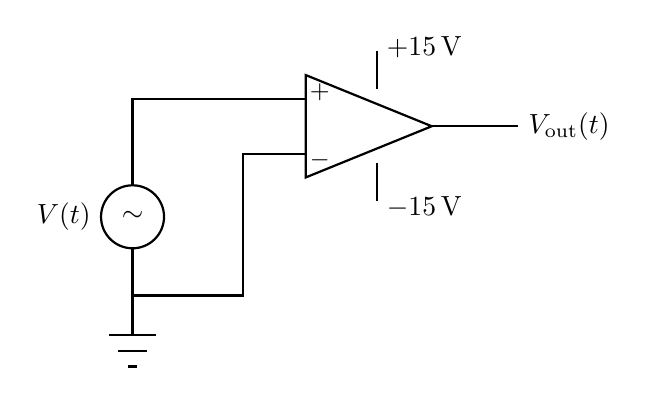
\begin{tikzpicture}[scale=1.0, thick]

  % AC source circle
  \draw (0,0) circle (0.4);
  \node at (0,0) {$\sim$};
  \node[left] at (-0.4,0) {$V(t)$};

  % wire from top of source to + terminal of opamp
  \draw (0,0.4) -- (0,1.5) -- (2.2,1.5);

  % feedback wire from - terminal back to bottom of source
  \draw (2.2,0.8) -- (1.4,0.8) -- (1.4,-1.0) -- (0,-1.0) -- (0,-0.4);

  % ground symbol
  \draw (0,-1.0) -- (0,-1.5);
  \draw (-0.3,-1.5) -- (0.3,-1.5);
  \draw (-0.18,-1.7) -- (0.18,-1.7);
  \draw (-0.06,-1.9) -- (0.06,-1.9);

  % Op-amp triangle
  \draw (2.2,1.8) -- (2.2,0.5) -- (3.8,1.15) -- cycle;
  \node at (2.38,1.58) {\small $+$};
  \node at (2.38,0.72) {\small $-$};

  % +15V supply line
  \draw (3.1,1.62) -- (3.1,2.1);
  \node[right] at (3.1,2.15) {$+15\,\text{V}$};

  % -15V supply line
  \draw (3.1,0.68) -- (3.1,0.2);
  \node[right] at (3.1,0.12) {$-15\,\text{V}$};

  % Output wire
  \draw (3.8,1.15) -- (4.9,1.15);
  \node[right] at (4.9,1.15) {$V_{\mathrm{out}}(t)$};

\end{tikzpicture}
\end{center}
\\
\hline
 & \\
\hline
(A) & $V_{\mathrm{out}}(t)$ is square wave with peak-to-peak voltage $= 30\,\text{V}$ and time period is $1\,\text{ms}$. \\
\hline
(B) & $V_{\mathrm{out}}(t)$ is a sine wave with peak-to-peak voltage $= 4\,\text{V}$ and time period is $1\,\text{ms}$. \\
\hline
(C) & $V_{\mathrm{out}}(t)$ is sine wave with peak-to-peak voltage $= 30\,\text{V}$ and time period of $1\,\text{ms}$. \\
\hline
(D) & $V_{\mathrm{out}}(t)$ is square wave with peak-to-peak voltage $= 4\,\text{V}$ and time period is $1\,\text{ms}$. \\
\hline
 & \\
\hline
\end{tabular}
\end{table}

\clearpage

\vspace{0.4cm}

\begin{table}[h]
\begin{tabular}{|L|C|}
\hline
Q.44 &
Considering the circuit and the associated signals measured at different pins (numbered as
1, 2, 3, 4, 5) shown in the figure, the correct option is

\vspace{0.3cm}
\begin{center}
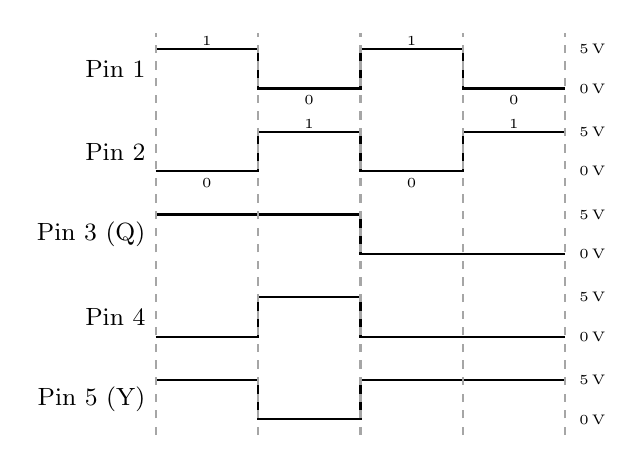
\begin{tikzpicture}[scale=1.0, thick]

%% ── Timing diagram (right) ────────────────────
\begin{scope}[xshift=6.2cm, yshift=-0.3cm]

  \def\T{1.3}
  \def\h{0.5}
  \def\g{1.05}

  % Pin 1 (P): 1 0 1 0
  \node[left] at (0,4*\g+\h/2) {\small Pin 1};
  \node[right] at (4*\T+0.05,4*\g+\h) {\tiny 5\,V};
  \node[right] at (4*\T+0.05,4*\g)    {\tiny 0\,V};
  \draw (0,4*\g+\h) -- (\T,4*\g+\h) -- (\T,4*\g)
        -- (2*\T,4*\g) -- (2*\T,4*\g+\h) -- (3*\T,4*\g+\h)
        -- (3*\T,4*\g) -- (4*\T,4*\g);
  \node at (0.5*\T,4*\g+\h+0.1) {\tiny 1};
  \node at (1.5*\T,4*\g-0.15)   {\tiny 0};
  \node at (2.5*\T,4*\g+\h+0.1) {\tiny 1};
  \node at (3.5*\T,4*\g-0.15)   {\tiny 0};

  % Pin 2 (NOT P): 0 1 0 1
  \node[left] at (0,3*\g+\h/2) {\small Pin 2};
  \node[right] at (4*\T+0.05,3*\g+\h) {\tiny 5\,V};
  \node[right] at (4*\T+0.05,3*\g)    {\tiny 0\,V};
  \draw (0,3*\g) -- (\T,3*\g) -- (\T,3*\g+\h)
        -- (2*\T,3*\g+\h) -- (2*\T,3*\g) -- (3*\T,3*\g)
        -- (3*\T,3*\g+\h) -- (4*\T,3*\g+\h);
  \node at (0.5*\T,3*\g-0.15)   {\tiny 0};
  \node at (1.5*\T,3*\g+\h+0.1) {\tiny 1};
  \node at (2.5*\T,3*\g-0.15)   {\tiny 0};
  \node at (3.5*\T,3*\g+\h+0.1) {\tiny 1};

  % Pin 3 (Q): 1 1 0 0
  \node[left] at (0,2*\g+\h/2) {\small Pin 3 (Q)};
  \node[right] at (4*\T+0.05,2*\g+\h) {\tiny 5\,V};
  \node[right] at (4*\T+0.05,2*\g)    {\tiny 0\,V};
  \draw (0,2*\g+\h) -- (2*\T,2*\g+\h) -- (2*\T,2*\g) -- (4*\T,2*\g);

  % Pin 4: 0 1 0 0
  \node[left] at (0,1*\g+\h/2) {\small Pin 4};
  \node[right] at (4*\T+0.05,1*\g+\h) {\tiny 5\,V};
  \node[right] at (4*\T+0.05,1*\g)    {\tiny 0\,V};
  \draw (0,1*\g) -- (\T,1*\g) -- (\T,1*\g+\h)
        -- (2*\T,1*\g+\h) -- (2*\T,1*\g) -- (4*\T,1*\g);

  % Pin 5 (Y): 1 0 1 1
  \node[left] at (0,\h/2) {\small Pin 5 (Y)};
  \node[right] at (4*\T+0.05,\h) {\tiny 5\,V};
  \node[right] at (4*\T+0.05,0)  {\tiny 0\,V};
  \draw (0,\h) -- (\T,\h) -- (\T,0)
        -- (2*\T,0) -- (2*\T,\h) -- (4*\T,\h);

  % Vertical dashed lines
  \draw[dashed,gray!70] (0,-0.2)    -- (0,4*\g+\h+0.2);
  \draw[dashed,gray!70] (1*\T,-0.2) -- (1*\T,4*\g+\h+0.2);
  \draw[dashed,gray!70] (2*\T,-0.2) -- (2*\T,4*\g+\h+0.2);
  \draw[dashed,gray!70] (3*\T,-0.2) -- (3*\T,4*\g+\h+0.2);
  \draw[dashed,gray!70] (4*\T,-0.2) -- (4*\T,4*\g+\h+0.2);

\end{scope}

\end{tikzpicture}
\end{center}
\\
\hline
 & \\
\hline
(A) & NOT gate between pins 1 and 2 is faulty. \\
\hline
(B) & NOR gate is faulty. \\
\hline
(C) & NOT gate between pins 4 and 5 is faulty. \\
\hline
(D) & The NOR and output NOT gates, are both faulty. \\
\hline
 & \\
\hline
\end{tabular}
\end{table}

\clearpage
\begin{table}[h!]
\begin{tabular}{|L|C|}
\hline
Q.45 &
A gas of $N$ classical particles that can occupy energy levels $\epsilon_1$ and
$\epsilon_2 = \epsilon_1 + \Delta$ is in equilibrium with a reservoir at temperature $T$.
From the schematics shown below, choose the correct dependence of the internal energy
$U$ on $T$. \\
\hline
 & \\
\hline
(A) &
\begin{tikzpicture}[scale=0.7]
  \draw[->] (0,0) -- (3.5,0) node[right] {$T$};
  \draw[->] (0,0) -- (0,2.5) node[above] {$U$};
  \draw[thick] (0.1,0.1) .. controls (0.3,0.5) and (0.7,1.5) .. (1.2,2.0)
               .. controls (1.8,2.3) and (2.5,2.4) .. (3.2,2.45);
\end{tikzpicture} \\
\hline
(B) &
\begin{tikzpicture}[scale=0.7]
  \draw[->] (0,0) -- (3.5,0) node[right] {$T$};
  \draw[->] (0,0) -- (0,2.5) node[above] {$U$};
  \draw[thick] (0.1,0.05) .. controls (1.2,0.1) and (2.0,0.8) .. (2.6,1.8)
               .. controls (2.9,2.2) and (3.1,2.4) .. (3.2,2.45);
\end{tikzpicture} \\
\hline
(C) &
\begin{tikzpicture}[scale=0.7]
  \draw[->] (0,0) -- (3.5,0) node[right] {$T$};
  \draw[->] (0,0) -- (0,2.5) node[above] {$U$};
  \draw[thick] (0.1,2.4) .. controls (0.3,2.0) and (0.5,1.2) .. (0.8,0.6)
               .. controls (1.2,0.25) and (2.0,0.15) .. (3.2,0.1);
\end{tikzpicture} \\
\hline
(D) &
\begin{tikzpicture}[scale=0.7]
  \draw[->] (0,0) -- (3.5,0) node[right] {$T$};
  \draw[->] (0,0) -- (0,2.5) node[above] {$U$};
  \draw[thick] (0.1,0.05) -- (0.7,0.05)
               .. controls (1.2,0.08) and (1.8,0.6) .. (2.3,1.6)
               .. controls (2.7,2.1) and (3.0,2.3) .. (3.2,2.45);
\end{tikzpicture} \\
\hline
 & \\
\hline
\end{tabular}
\end{table}

\begin{table}[h!]
\begin{tabular}{|L|C|}
\hline
Q.46 &
The Lagrangian
\[
L_0 = \frac{1}{2}m\dot{q}^2 - \frac{1}{2}m\omega^2 q^2
\]
with the generalized coordinate $q$ is transformed to $L = L_0 + \alpha\dfrac{df(q)}{dt}$.
Consider the following statements:

\medskip
(i)\; Expression for the canonical momentum does not change.

(ii) The equation of the motion does not change.

\medskip
Which of the following options is correct for the above statements? \\
\hline
 & \\
\hline
(A) & Both (i) and (ii) are correct. \\
\hline
(B) & Both (i) and (ii) are not correct. \\
\hline
(C) & (i) is correct and (ii) is not correct. \\
\hline
(D) & (i) is not correct and (ii) is correct. \\
\hline
 & \\
\hline
\end{tabular}
\end{table}

\vspace{0.4cm}

\begin{table}[h!]
\begin{tabular}{|L|C|}
\hline
Q.47 &
An infinitely large thin sheet in the $xy$-plane carries uniform positive charge density
and is moving with constant velocity $\vec{v}$ in the $+x$ direction (see figure below).
The direction of the corresponding Poynting vector is

\vspace{0.3cm}
\begin{center}
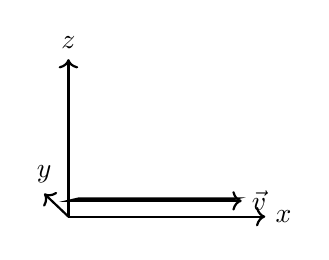
\begin{tikzpicture}[scale=1.0, thick]
  % axes
  \draw[->] (0,0,0) -- (2.5,0,0) node[right] {$x$};
  \draw[->] (0,0,0) -- (0,2.0,0) node[above] {$z$};
  \draw[->] (0,0,0) -- (0,0.6,0.8) node[above] {$y$};

  % sheet parallelogram
  \draw (0,0.2,0) -- (2.0,0.2,0) -- (2.4,0.5,0.7) -- (0.4,0.5,0.7) -- cycle;

  % velocity arrow
  \draw[->] (1.2,0.2,0) -- (2.2,0.2,0) node[right] {$\vec{v}$};
\end{tikzpicture}
\end{center}
\\
\hline
 & \\
\hline
(A) & $+x$ for both $z < 0$ and $z > 0$ \\
\hline
(B) & $+x$ for $z < 0$ and $-x$ for $z > 0$ \\
\hline
(C) & $-x$ for $z < 0$ and $+x$ for $z > 0$ \\
\hline
(D) & $-x$ for both $z < 0$ and $z > 0$ \\
\hline
 & \\
\hline
\end{tabular}
\end{table}

\vspace{0.4cm}

\begin{table}[h!]
\begin{tabular}{|L|C|}
\hline
Q.48 &
A positive point charge is fixed at the origin. At some distance from it on the $x$ axis,
a point dipole is kept pointing in the $+y$ direction. The force on the dipole is \\
\hline
 & \\
\hline
(A) & $0$ \\
\hline
(B) & in the $+y$ direction \\
\hline
(C) & in the $-y$ direction \\
\hline
(D) & in the $+x$ direction \\
\hline
 & \\
\hline
\end{tabular}
\end{table}

\vspace{0.4cm}

\begin{table}[h!]
\begin{tabular}{|L|C|}
\hline
Q.49 &
Two frames $S$ (solid lines) and $S'$ (dashed lines) with common origin are shown in the
figure below. Frame $S$ is inertial while $S'$ is rotating about the common $z$-axis.
There is a point mass fixed at $P$ on the $x$-axis of the $S$ frame. The magnitude of
the centrifugal force and the Coriolis force experienced by the mass in the $S'$ frame
is $F_{cen}$ and $F_{cor}$, respectively. Which of the following options is correct for
these forces?

\vspace{0.3cm}
\begin{center}
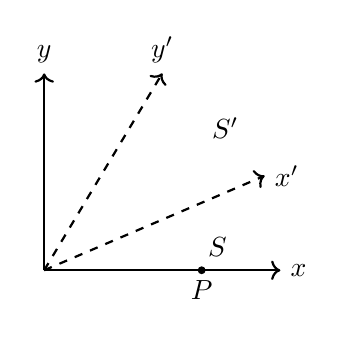
\begin{tikzpicture}[scale=1.0, thick]
  % S frame axes (solid)
  \draw[->] (0,0) -- (3.0,0) node[right] {$x$};
  \draw[->] (0,0) -- (0,2.5) node[above] {$y$};

  % S' frame axes (dashed)
  \draw[->, dashed] (0,0) -- (1.5,2.5) node[above] {$y'$};
  \draw[->, dashed] (0,0) -- (2.8,1.2) node[right] {$x'$};

  % S' label
  \node at (2.3,1.8) {$S'$};
  % S label
  \node at (2.2,0.3) {$S$};

  % Point P on x-axis
  \fill (2.0,0) circle (0.05);
  \node[below] at (2.0,0) {$P$};
\end{tikzpicture}
\end{center}
\\
\hline
 & \\
\hline
(A) & $F_{cen} = 0$ and $F_{cor} = 0$ \\
\hline
(B) & $F_{cen} \neq 0$ and $F_{cor} \neq 0$ and $F_{cen} = \dfrac{F_{cor}}{2}$ \\
\hline
(C) & $F_{cen} \neq 0$ and $F_{cor} \neq 0$ and $F_{cen} = 2F_{cor}$ \\
\hline
(D) & $F_{cen} \neq 0$ and $F_{cor} \neq 0$ and $F_{cen} = F_{cor}$ \\
\hline
 & \\
\hline
\end{tabular}
\end{table}

\vspace{0.4cm}

\begin{table}[h!]
\begin{tabular}{|L|C|}
\hline
Q.50 &
Which of the following operators is/are self-adjoint? \\
\hline
 & \\
\hline
(A) & \rule{0pt}{1.2cm} $x^2\dfrac{d^2}{dx^2} + 3x\dfrac{d}{dx} + x^2$ \\
\hline
(B) & \rule{0pt}{1.2cm} $(1-x^2)\dfrac{d^2}{dx^2} - 2x\dfrac{d}{dx} + 3x$ \\
\hline
(C) & \rule{0pt}{1.2cm} $(3x - 4x^3)\dfrac{d^2}{dx^2} + (3 - 12x^2)\dfrac{d}{dx} + 12$ \\
\hline
(D) & \rule{0pt}{1.2cm}$x\dfrac{d^2}{dx^2} + x^2\dfrac{d}{dx} + \dfrac{5x}{3}$ \\
\hline
 & \\
\hline
\end{tabular}
\end{table}

\vspace{0.4cm}

\begin{table}[h!]
\begin{tabular}{|L|C|}
\hline
Q.51 &
Consider two operators $\hat{A}$ and $\hat{B}$ which are related as
$\hat{A} = \exp(i\theta\hat{B})$. If $\theta$ is a non-zero real number, which of the
following statements is/are true? \\
\hline
 & \\
\hline
(A) & If $\hat{B}$ is Hermitian, then $\hat{A}$ is unitary. \\
\hline
(B) & If $\hat{B}$ is anti-Hermitian, then $\hat{A}$ is unitary. \\
\hline
(C) & If $\hat{B}$ is Hermitian, then $|Det(\hat{A})| = 1$. \\
\hline
(D) & If $\hat{B}$ is anti-Hermitian, then $\hat{A}$ is Hermitian. \\
\hline
 & \\
\hline
\end{tabular}
\end{table}

\clearpage

%-----------------------------
% Q.52
%-----------------------------
\begin{table}[h!]
\begin{tabular}{|p{0.08\textwidth}|p{0.82\textwidth}|}
\hline
\textbf{Q.52} &
Consider operators $\hat{A}$, $\hat{B}$, and $\hat{C}$ for three observables of a quantum system satisfying $[\hat{A}, \hat{B}] = 0$, $[\hat{B}, \hat{C}] = 0$, and $[\hat{A}, \hat{C}] \neq 0$, with uncertainties $\Delta A$, $\Delta B$, $\Delta C$, respectively. From the options given below, which is/are implied by the commutation relations among $\hat{A}$, $\hat{B}$, and $\hat{C}$? \\
\hline
& \\
\hline
(A) & $\Delta A\, \Delta B > 0$ \\
\hline
(B) & $\Delta A\, \Delta C > 0$ \\
\hline
(C) & $\hat{A}$, $\hat{B}$ can be simultaneously diagonalized. \\
\hline
(D) & $\hat{A}$, $\hat{B}$, $\hat{C}$ can be simultaneously diagonalized. \\
\hline
& \\
\hline
\end{tabular}
\end{table}

\bigskip

%-----------------------------
% Q.53
%-----------------------------
\begin{table}[h!]
\begin{tabular}{|p{0.08\textwidth}|p{0.82\textwidth}|}
\hline
\textbf{Q.53} &
Consider the distribution of outcomes generated by $N$ ($N \gg 1$) independent throws of (i) a coin or (ii) a six-sided dice. A coin (dice) is unbiased if both (all) its sides have equal probability to show up in a throw; it is biased otherwise. For the cases (i) and (ii) above, which of the following statements is/are true? \\
\hline
& \\
\hline
(A) & The entropy of an unbiased coin is smaller than that of an unbiased dice. \\
\hline
(B) & The entropy of an unbiased coin is greater than that of an unbiased dice. \\
\hline
(C) & The entropy of a biased dice is smaller than that of an unbiased dice. \\
\hline
(D) & The entropy of a biased coin is greater than that of an unbiased coin. \\
\hline
& \\
\hline
\end{tabular}
\end{table}

\clearpage

%-----------------------------
% Q.54
%-----------------------------
\begin{table}[h!]
\begin{tabular}{|p{0.08\textwidth}|p{0.82\textwidth}|}
\hline
\textbf{Q.54} &
The dispersion $(E(k))$ of the conduction band (CB) and valence band (VB) for a semiconductor are shown schematically in the figure. Considering the possibility of an electron making a transition from the bottom of the CB to the top of the VB, which of the following options is/are correct?

\vspace{0.3cm}
\begin{center}
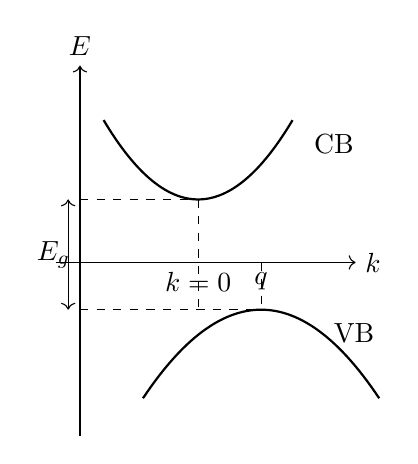
\begin{tikzpicture}[scale=1.0]
  % Axes
  \draw[->] (0,-2.2) -- (0,2.5) node[above] {$E$};
  \draw[->] (-0.3,0) -- (3.5,0) node[right] {$k$};
  % CB: parabola opening upward, minimum at k=0
  \draw[thick] plot[domain=-1.2:1.2, samples=60] ({1.5+\x}, {0.8 + 0.7*\x*\x});
  \node[right] at (2.85,1.5) {CB};
  % VB: parabola opening downward, maximum at k=q (shifted right)
  \draw[thick] plot[domain=-1.5:1.5, samples=60] ({1.5+\x+0.8}, {-0.6 - 0.5*\x*\x});
  \node[right] at (3.1,-0.9) {VB};
  % Dashed lines for Eg
  \draw[dashed] (0,0.8) -- (1.5,0.8);
  \draw[dashed] (0,-0.6) -- (2.3,-0.6);
  % Eg brace
  \draw[dashed] (1.5,0.8) -- (1.5,-0.6);
  \node[left] at (0,0.1) {$E_g$};
  \draw[<->] (-0.15,-0.6) -- (-0.15,0.8);
  % k=0 and q labels
  \node[below] at (1.5,0) {$k=0$};
  \draw[dashed] (2.3,0) -- (2.3,-0.6);
  \node[below] at (2.3,0) {$q$};
\end{tikzpicture}
\end{center}
\\
\hline
(A) & The transition is forbidden. \\
\hline
(B) & A photon can be emitted with an energy exactly equal to $E_g$. \\
\hline
(C) & A photon can be emitted with an energy less than $E_g$. \\
\hline
(D) & A phonon can be created with a crystal momentum $\hbar q$. \\
\hline
& \\
\hline
\end{tabular}
\end{table}

\clearpage
\newpage

%-----------------------------
% Q.55
%-----------------------------
\begin{table}[h!]
\begin{tabular}{|p{0.08\textwidth}|p{0.82\textwidth}|}
\hline
\textbf{Q.55} &
A symmetric rigid body has moment of inertia $I_1$, $I_2$, $I_3$ about its principal axes 1, 2, and 3, respectively, with $I_1 = I_2 = I_\perp$ and $I_3 \neq I_\perp$. It is rotating in space with no torque on it so that its angular momentum $\vec{L}$ is constant. Let $\omega_1, \omega_2, \omega_3$ be the components of its angular velocity along the principal axes 1, 2, and 3, respectively. Which of the following quantities is/are constant during the motion of this rigid body? \\
\hline
(A) & $\omega_1 + \omega_3$ \\
\hline
(B) & $\omega_1^2 + \omega_3^2$ \\
\hline
(C) & Angle between axis 2 and $\vec{L}$ \\
\hline
(D) & $\omega_2$ \\
\hline
& \\
\hline
\end{tabular}
\end{table}

\bigskip

%-----------------------------
% Q.56
%-----------------------------
\begin{table}[h!]
\begin{tabular}{|p{0.08\textwidth}|p{0.82\textwidth}|}
\hline
\textbf{Q.56} &
An $\alpha$ particle moves towards a fixed nucleus carrying charge $Ze$, with initial speed $v_0$ and impact parameter $b$. Starting from a large distance from the nucleus, its distance of closest approach is $r_m$ and its speed there is $v_m$. Then which of the following options is/are correct?
\[
\left(k = \frac{1}{4\pi\epsilon_0}\ \text{ and }\ r_0 = k\frac{2Ze^2}{mv_0^2}\right)
\] \\
\hline
(A) & \rule{0pt}{1.2cm} $v_0 b = v_m r_m$ \\[8pt]
\hline
(B) & \rule{0pt}{1.2cm} $v_0 b = 2v_m r_0$ \\[8pt]
\hline
(C) & \rule{0pt}{1.2cm}  For $\dfrac{b}{r_0} \ll 1$,\ $r_m = 4r_0 + \dfrac{b^2}{2r_0}$\ ignoring higher order corrections in $\dfrac{b}{r_0}$ \\[8pt]
\hline
(D) & \rule{0pt}{1.2cm} For $\dfrac{b}{r_0} \ll 1$,\ $r_m = 4r_0 + \dfrac{b^2}{8r_0}$\ ignoring higher order corrections in $\dfrac{b}{r_0}$ \\[8pt]
\hline
& \\
\hline
\end{tabular}
\end{table}

\newpage

%-----------------------------
% Q.57
%-----------------------------
\begin{table}[h!]
\begin{tabular}{|p{0.08\textwidth}|p{0.82\textwidth}|}
\hline
\textbf{Q.57} &
Consider a particle of mass $m = 9.0 \times 10^{-5}$ kg and charge $q = 3.0 \times 10^{-4}$ C in a uniform electromagnetic field $\vec{E} = 2\,\hat{x}$ V$\cdot$m$^{-1}$, $\vec{B} = 3\,\hat{z}$ V$\cdot$m$^{-2}$s. The particle is released from the coordinates $(0,\,5\,\text{m},\,0)$ at time $t = 0$. Starting from initial speed zero, it comes back to the $y$-axis for the first time at time $t$. The value of $t$ in seconds (rounded off to two decimal places) is \underline{\hspace{1.5cm}}. \\
\hline
\end{tabular}
\end{table}

\bigskip

%-----------------------------
% Q.58
%-----------------------------
\begin{table}[h!]
\begin{tabular}{|p{0.08\textwidth}|p{0.82\textwidth}|}
\hline
\textbf{Q.58} &
An atom has two energy levels with energy difference 2.2 eV between them. A gas of these atoms is with $8 \times 10^{20}$ atoms in the upper state and $5 \times 10^{20}$ atoms in the lower state. Ignoring spontaneous emission, the maximum possible energy released by this gas of atoms by stimulated emission is $E$ Joules. The value of $E$ (rounded off to one decimal place) is \underline{\hspace{1.5cm}}.

\medskip
$(e = 1.6 \times 10^{-19}$ C$)$ \\
\hline
\end{tabular}
\end{table}

\bigskip

%-----------------------------
% Q.59
%-----------------------------
\begin{table}[h!]
\begin{tabular}{|p{0.08\textwidth}|p{0.82\textwidth}|}
\hline
\textbf{Q.59} &
The Hamiltonian of two interacting spin-1/2 particles is $H = \dfrac{A}{\hbar^2}\,\vec{S}_1 \cdot \vec{S}_2$, where $\vec{S}_1$ and $\vec{S}_2$ are the spin angular momenta of particles 1 and 2, respectively. Here, $A = 10.56$ eV. The energy in eV required to induce an excitation from the ground state to the excited state (rounded off to two decimal places) is \underline{\hspace{1.5cm}}. \\
\hline
\end{tabular}
\end{table}

\newpage

\newpage
%-----------------------------
% Q.60
%-----------------------------
\begin{table}[h!]
\begin{tabular}{|p{0.08\textwidth}|p{0.82\textwidth}|}
\hline
\textbf{Q.60} &
The output signal (current $I_d$) of a reversed biased (with a voltage $V_b$) photodiode, on which light is incident, is fed to an amplifier (see figure). The output voltage is digitized by a 10 bit Analogue to Digital Convertor (ADC) which has a reference voltage of 5 V. The smallest current $I_d$ which can be measured by the circuit in nano-Amperes (rounded off to one decimal place) is \underline{\hspace{1.5cm}}.
\vspace{0.4cm}
\begin{center}
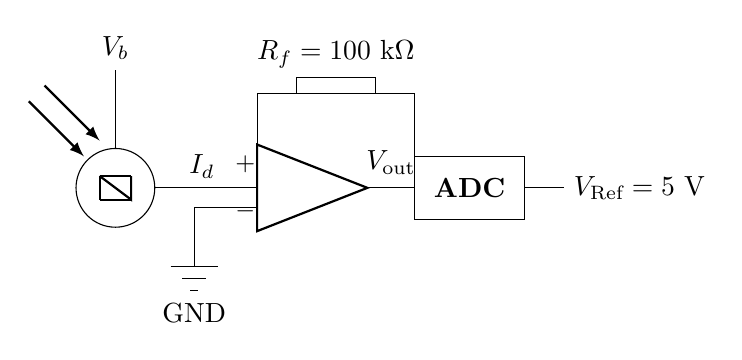
\begin{tikzpicture}[scale=1.0, >=latex]
  % Photodiode circle
  \draw (0,0) circle (0.5);
  % Light arrows hitting diode
  \draw[->, thick] (-1.1,1.1) -- (-0.4,0.4);
  \draw[->, thick] (-0.9,1.3) -- (-0.2,0.6);
  % Vb wire going up
  \draw (0,0.5) -- (0,1.5) node[above] {$V_b$};
  % Diode symbol inside circle
  \draw[thick] (-0.2,-0.15) -- (0.2,-0.15);
  \draw[thick] (-0.2,0.15) -- (0.2,0.15);
  \draw[thick] (-0.2,0.15) -- (-0.2,-0.15);
  \draw[thick] (-0.2,0.15) -- (0.2,-0.15) -- (0.2,0.15);
  % Wire right from diode to op-amp - input
  \draw (0.5,0) -- (1.8,0) -- (1.8,-0.25);
  \node[above] at (1.1,0) {$I_d$};
  % Op-amp
  \draw[thick] (1.8,0.55) -- (1.8,-0.55) -- (3.2,0) -- cycle;
  \node at (1.65,0.3) {\small $+$};
  \node at (1.65,-0.3) {\small $-$};
  % GND on minus input
  \draw (1.8,-0.25) -- (1.0,-0.25) -- (1.0,-1.0);
  \draw (0.7,-1.0) -- (1.3,-1.0);
  \draw (0.85,-1.15) -- (1.15,-1.15);
  \draw (0.95,-1.3) -- (1.05,-1.3);
  \node[below] at (1.0,-1.35) {GND};
  % Feedback resistor on top
  \draw (1.8,0.3) -- (1.8,1.2) -- (3.8,1.2) -- (3.8,0);
  % Resistor box in feedback
  \draw (2.3,1.2) -- (2.3,1.4) -- (3.3,1.4) -- (3.3,1.2);
  \node[above] at (2.8,1.4) {$R_f = 100\ \text{k}\Omega$};
  % Output wire
  \draw (3.2,0) -- (3.8,0);
  \node[above] at (3.5,0.05) {$V_{\text{out}}$};
  % ADC box
  \draw (3.8,-0.4) rectangle (5.2,0.4);
  \node at (4.5,0) {\textbf{ADC}};
  % Vref wire
  \draw (5.2,0) -- (5.7,0) node[right] {$V_{\text{Ref}} = 5\ \text{V}$};
\end{tikzpicture}
\end{center}
\\
\hline
\end{tabular}
\end{table}
\newpage

%-----------------------------
% Q.61
%-----------------------------
\begin{table}[h!]
\begin{tabular}{|p{0.08\textwidth}|p{0.82\textwidth}|}
\hline
\textbf{Q.61} &
A capacitor is made of two circular metal plates of radius 1 m separated by a distance $d = 1$ mm. The space between them is filled by a dielectric with permittivity $\epsilon_r = 5$. The capacitor is connected to a voltage $V = 10\sin(2\pi \times 10^6 \times t)$ volts, where $t$ is in seconds. The maximum value of the magnetic field in between the plates at a radial distance $r = 0.5$ m from the centre of the capacitor is $B \times 10^{-6}$ T. The value of $B$ (rounded off to two decimal places) is \underline{\hspace{1.5cm}}.

\medskip
(Speed of light in vacuum $c = 3 \times 10^8$ m$\cdot$s$^{-1}$) \\
\hline
\end{tabular}
\end{table}

\bigskip

%-----------------------------
% Q.62
%-----------------------------
\begin{table}[h!]
\begin{tabular}{|p{0.08\textwidth}|p{0.82\textwidth}|}
\hline
\textbf{Q.62} &
Rotational spectrum of a diatomic molecule consists of lines of equal spacing with an interval of 20.0 cm$^{-1}$. Its moment of inertia is found to be $I_0 \times 10^{-47}$ kg$\cdot$m$^2$, the value of $I_0$ (rounded off to one decimal place) is \underline{\hspace{1.5cm}}.

\medskip
$(h = 6.6 \times 10^{-34}$ J$\cdot$s, speed of light in vacuum $c = 3 \times 10^8$ m$\cdot$s$^{-1})$ \\
\hline
\end{tabular}
\end{table}

\bigskip

%-----------------------------
% Q.63
%-----------------------------
\begin{table}[h!]
\begin{tabular}{|p{0.08\textwidth}|p{0.82\textwidth}|}
\hline
\textbf{Q.63} &
Copper has an electron number density of $8.3 \times 10^{28}$ m$^{-3}$. Its Fermi energy in eV (rounded off to one decimal place) is \underline{\hspace{1.5cm}}.

\medskip
$(h = 1.06 \times 10^{-34}$ J$\cdot$s, mass of electron $m_e = 9.10 \times 10^{-31}$ kg, charge of electron $= 1.60 \times 10^{-19}$ C$)$ \\
\hline
\end{tabular}
\end{table}

\newpage

%-----------------------------
% Q.64
%-----------------------------
\begin{table}[h!]
\begin{tabular}{|p{0.08\textwidth}|p{0.82\textwidth}|}
\hline
\textbf{Q.64} &
Two 1 kg blocks are connected to two massless springs of spring constants 8 N$\cdot$m$^{-1}$ and 4 N$\cdot$m$^{-1}$. The system is kept on a frictionless horizontal floor with one end of a spring attached to a wall (see figure below). They are performing oscillatory motion along the $x$-axis with the normal mode frequencies $\omega_H$ and $\omega_L$ $(\omega_H > \omega_L)$. The ratio $\dfrac{\omega_H}{\omega_L}$ (rounded off to two decimal places) is \underline{\hspace{1.5cm}}.

\vspace{0.4cm}
\begin{center}
\begin{tikzpicture}[>=latex, scale=1.1]
  % Wall
  \fill[gray!50] (-0.3,-0.6) rectangle (0,0.6);
  \draw[thick] (0,-0.6) -- (0,0.6);
  \foreach \y in {-0.5,-0.3,-0.1,0.1,0.3,0.5}
    \draw (-0.3,\y) -- (0,\y+0.2);
  % Spring 1
  \draw[thick, decoration={coil, coil aspect=0.4, segment length=5pt, amplitude=5pt},
        decorate] (0,0) -- (2.0,0);
  \node[above] at (1.0,0.35) {$8\ \text{N.m}^{-1}$};
  % Block 1
  \draw[thick, fill=gray!40] (2.0,-0.35) rectangle (2.8,0.35);
  % Spring 2
  \draw[thick, decoration={coil, coil aspect=0.4, segment length=5pt, amplitude=5pt},
        decorate] (2.8,0) -- (4.8,0);
  \node[above] at (3.8,0.35) {$4\ \text{N.m}^{-1}$};
  % Block 2
  \draw[thick, fill=gray!40] (4.8,-0.35) rectangle (5.6,0.35);
  % x-axis arrow
  \draw[->] (5.8,0) -- (6.4,0) node[right] {$x$};
\end{tikzpicture}
\end{center}
\\
\hline
\end{tabular}
\end{table}

\newpage

\bigskip



%-----------------------------
% Q.65
%-----------------------------
\begin{table}[h!]
\begin{tabular}{|p{0.08\textwidth}|p{0.82\textwidth}|}
\hline
\textbf{Q.65} &
A 15 cm long scale is held horizontally with one of its ends on the edge of a 1 m high table and the other end resting on one's index finger. As the finger is removed (see figure below), the scale starts rotating about its end on the table. After 0.1 s, during which it has rotated by a negligibly small angle but has gained a rotational speed as it leaves the table and falls vertically towards the ground. When its centre of mass has fallen by 0.5 m, it has rotated by an angle $\theta$. The value of $\theta$ in degrees (rounded off to one decimal place) is \underline{\hspace{1.5cm}}.

\medskip
$(g = 9.8\ \text{m.s}^{-2})$

\vspace{0.4cm}
\begin{center}
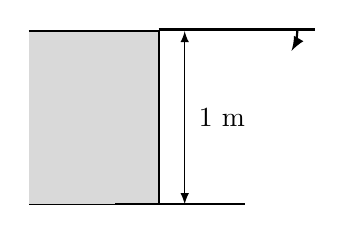
\begin{tikzpicture}[>=latex, scale=1.1]
  % Table top surface
  \draw[thick] (-1.5,0) -- (0,0);
  % Table edge (vertical)
  \draw[thick] (0,0) -- (0,-2.0);
  % Table bottom
  \draw[thick] (-1.5,-2.0) -- (0,-2.0);
  % Hatch for table
  \fill[gray!30] (-1.5,-2.0) rectangle (0,0);
  \draw[thick] (-1.5,0) -- (0,0);
  \draw[thick] (0,0) -- (0,-2.0);
  % Scale on table (horizontal, extending right)
  \draw[very thick] (0,0.02) -- (1.8,0.02);
  % Arrow showing rotation direction
  \draw[->, thick] (1.6,0.02) arc[start angle=0, end angle=-30, radius=0.5];
  % 1 m height label
  \draw[<->] (0.3,0) -- (0.3,-2.0);
  \node[right] at (0.35,-1.0) {1 m};
  % Ground
  \draw[thick] (-0.5,-2.0) -- (1.0,-2.0);
\end{tikzpicture}
\end{center}
\\
\hline
\end{tabular}
\end{table}

\end{document}
